%% LaTeX2e class for student theses
%% sections/content.tex
%% 
%% Karlsruhe Institute of Technology
%% Institute of Information Security and Dependability (KASTEL)
%%
%% Template by
%% Dr.-Ing. Erik Burger
%% burger@kit.edu
%%
%% Adaption by
%% Annika Vielsack
%% vielsack@kit.edu
%%
%% Version 1.0, 2021-07-03

\chapter{Preliminary Knowledge}
\label{ch:Backgroud}

\definecolor{codegreen}{rgb}{0,0.6,0}
\definecolor{codegray}{rgb}{0.5,0.5,0.5}
\definecolor{codepurple}{rgb}{0.58,0,0.82}
\definecolor{backcolour}{rgb}{0.95,0.95,0.92}

\lstdefinestyle{mystyle}{
    backgroundcolor=\color{backcolour},   
    commentstyle=\color{codegreen},
    keywordstyle=\color{magenta},
    numberstyle=\tiny\color{codegray},
    stringstyle=\color{codepurple},
    basicstyle=\ttfamily\footnotesize,
    breakatwhitespace=false,         
    breaklines=true,                 
    captionpos=b,                    
    keepspaces=true,                 
    numbers=left,                    
    numbersep=5pt,                  
    showspaces=false,                
    showstringspaces=false,
    showtabs=false,                  
    tabsize=2
}

\lstset{style=mystyle}












\chapter{Vulnerabilities and Real-world exploits in Solidity Smart Contracts}
\label{ch:SmartContracts}

\section{Most common Vulnerabilities}
\label{sec:SmartContracts:Vulnerabilities}
\subsection{Denial Of Services}
\label{sec:Vulnerabilities:DOS}
The article \citet{CloudFareDos} of CloudFare, proposes a definition of denial-of-service (DoS) attack. It is a type of cyber attack in 
which an attacker aims to render a computer or a informatic service (logical or phisical) unavailable to its intended users by interrupting the 
device's normal functioning. 

In Solidity contetext, DoS consists of attacks where 
users can leave the contract inoperable for a small period of time, or in some cases, permanently.
It represents a cathegory of attacks, consequently it is not possible to classify a 
spefic vulnerability or methodology for exploiting a thread.

As an example of this class of attack, I selected the smart contract presented by \citet{Dos1}. 
It allows the user to place a bid to the contract. If it is the highest bid, it 
sends the previous leader the current bid and set the leader to the sender with the new highest bid.
The vulnerability relies on line 12 (\refname{lst:DosContract1}): the require condition is respected if the transaction which refunds the old leader doesn not revert. 
An attacker can exploit this vulnerability, creating a smart contract which cannot receive ether. Then it intacts with the vulnerable contract, becoming the leader.
When the vulnerable tries to refund the attacker one, it will always revert because it cannot receive ether and no one could become the new leader.

\begin{lstlisting} [language={C++},caption={Dos Vulnerable Contract.}, label={lst:DosContract1}]
    pragma solidity ^0.8.0;

    /**
     * @title VulnerableContract
     * @dev This contract is vulnerable to a denial of service (DoS) attack
     */
    contract VulnerableContract {
        address payable leader;
        uint256 public highestBid;
    
        function bid() external payable {
            require(msg.value > highestBid);
    
            // Refund the old leader, if it fails then revert
            require(leader.send(highestBid));
    
            leader = payable(msg.sender);
            highestBid = msg.value;
        }
    
        /// Helper function to check leader
        function getLeader() external view returns (address) {
            return leader;
        }
    }
    
\end{lstlisting}

Another exapmle is 



\section{Real world Exploits}
\label{sec:SmartContracts:Exploits}
Real-wolrd exploits that have happend in the recent years.
\subsection{XSURGE on BSC Chain}
\label{sec:Exploits:XSURGE}

The \citet{XSurgeWeb}'s whitepaper provides a presentation of the ecosystem.
It is described as a great DeFi investing idea based on proprietary pricing algorithms embedded in the Surge Token Variants' contracts.
Surge Token Variants each have their own Market Maker, allowing them to trade continuously and outlast both 
centralised and decentralised exchanges. 
The strategy is to reward long-term holding by increasing a
holder's claim of the backing asset. Each Surge Token utilizes a built-in contract exchange system that renounces the need for
a traditional liquidity pool. Both assets are stored within the contract itself, 
rather than a liquidity pool pair of the backing asset to the
token using a traditional market maker method for exchange and price calculation.

One of the Surge Token is SurgeBNB, the one which is my focus of analysis.
\citet{XSurgeBNB} explains in deep how the attack to this contract occured. 
The Official claimed that the attacker had stolen \$5 million in SurgeBNB through a backdoor vulnerability.
XSURGE stated that a potential security vulnerability in the SurgeBNB contract was discovered on August 16th.

The attack is mabe by 4 main steps:
\begin{enumerate}
    \item the attacker borrow  10,000BNB through flash loans.
    \item Use all the BNB to buy SURGE. According to the current price, 
    the attacker can buy 1,896,594,328,449,690 SURGE
    \item He calls the "sell" function, for selling the obtained SURGE.
    \item The sale function alters the data after the transfer, and the transfer code has a reentrance vulnerability.
    When the attack contract acquires BNB, the period before the SURGE contract's state changes 
    (\refname{lst:SellSURGE} line 15 ), the attack contract can use the reentrance 
    vulnerability to purchase SURGE again.
\end{enumerate}

\begin{lstlisting} [language={C++},caption={Sell function of Surge (SURGE) token.}, label={lst:SellSURGE}]
    function sell(uint256 tokenAmount) public nonReentrant returns (bool) {
        
        address seller = msg.sender;
        
        // make sure seller has this balance
        require(_balances[seller] >= tokenAmount, 'cannot sell above token amount');
        
        // calculate the sell fee from this transaction
        uint256 tokensToSwap = tokenAmount.mul(sellFee).div(10**2);
        
        // how much BNB are these tokens worth?
        uint256 amountBNB = tokensToSwap.mul(calculatePrice());
        
        // send BNB to Seller
        (bool successful,) = payable(seller).call{value: amountBNB, gas: 40000}(""); 
        if (successful) {
            // subtract full amount from sender
            _balances[seller] = _balances[seller].sub(tokenAmount, 'sender does not have this amount to sell');
            // if successful, remove tokens from supply
            _totalSupply = _totalSupply.sub(tokenAmount);
        } else {
            revert();
        }
        emit Transfer(seller, address(this), tokenAmount);
        return true;
    }
\end{lstlisting}


The bnb Amount of the contract stays intact, and the total amount of SURGE tokens \texttt{ totalSupply }  
has not been updated, because the attack contract spends all of the BNB balance to acquire SURGE
 each time (still remains the quantity before the sell).
As a result, the price of token falls, allowing the attacker to purchase additional SURGE. 


\begin{lstlisting} [language={C++},caption={Purchase function of Surge (SURGE) token.}, label={lst:SellPurchase}]
    function purchase(address buyer, uint256 bnbAmount) internal returns (bool) {
        // make sure we don't buy more than the bnb in this contract
        require(bnbAmount <= address(this).balance, 'purchase not included in balance');
        // previous amount of BNB before we received any        
        uint256 prevBNBAmount = (address(this).balance).sub(bnbAmount);
        // if this is the first purchase, use current balance
        prevBNBAmount = prevBNBAmount == 0 ? address(this).balance : prevBNBAmount;
        // find the number of tokens we should mint to keep up with the current price
        uint256 nShouldPurchase = hyperInflatePrice ? _totalSupply.mul(bnbAmount).div(address(this).balance) : _totalSupply.mul(bnbAmount).div(prevBNBAmount);
        // apply our spread to tokens to inflate price relative to total supply
        uint256 tokensToSend = nShouldPurchase.mul(spreadDivisor).div(10**2);
        // revert if under 1
        if (tokensToSend < 1) {
            revert('Must Buy More Than One Surge');
        }
        
        // mint the tokens we need to the buyer
        mint(buyer, tokensToSend);
        emit Transfer(address(this), buyer, tokensToSend);
        return true;
    }
\end{lstlisting}

Repeating three times of Round 2 and Round 3 , the attacker accumulates a large amount of SURGE through reentry, and then sells all the SURGE to make a profit.

At the end of this transaction, the attack contract sold 1,864,120,345,279,610,000 SURGE, 
obtained 10327 BNB, and finally the profitable 297 BNB was sent to the attacker's address.

The following are the modifications suggested by the Beosin technical team for this attack:
\begin{itemize}
    \item any transfer operation should be place after the state changes to avoid reentry assaults.
    \item Instead of using "call. value," use transfer or send to transfer. 
\end{itemize}

\chapter{Analysis Tools}
\label{ch:Tools}
In this chapter I describe the tools and their capabilities, how they perform the Analysis.

\section{Typologies of Tools}
\label{sec:Tools:Typologies}
I explain the different types of analysis exsting in general, as Symbolic execution, formal specification, scanner, Symbolic execution.

\section{Tools for analysing properties specified by user}
\label{sec:Tools:Specification}
Description of tools, I would say like an overview of their papaer 

\subsection{Celestial}
\label{sec:Specification:Celestial}


\subsection{SmartPulse}
\label{sec:Specification:SmartPulse}

\subsection{VeriSol}
\label{sec:Specification:VeriSol}


\subsection{Echidna}
\label{sec:Specification:Echidna}
Echidna is an open-source smart contract fuzzer, developed by \citet{Echidna}, which makes it easy to automatically generate tests to detect violations in
assertions and custom properties.
Rather than relying on a fixed set of pre-defined bug oracles to detect vulnerabilities
during fuzzing campaigns, Echidna supports three types of proper-
ties: 
\begin{itemize}
    \item user-defined properties (for property-based testing;
    \item assertion checking;
    \item gas use estimation.
\end{itemize}

Figure \ref{fig:echdina_architecture} depicts the Echidna architecture as a two-step process: pre-processing and fuzzing.
The tool starts with a collection of contracts that have been supplied, as well as attributes that have been integrated into one of the contracts.
Echidna uses Slither , smart contract static analysis framework presenet in \ref{sec:WithoutSpecification:Slither}, to build and analyse the contracts in order to find relevant constants and functions that directly handle Ether (ETH).
The fuzzing effort begins in the second stage. 
Using the application binary interface (ABI) given by the contract, significant constants stated in the contract, 
and any previously gathered sets of transactions from the corpus, this iterative procedure creates random transactions. 
When a property violation is detected, a counterexample is created to indicate the smallest and most basic sequence of operations that caused the failure. 

\begin{figure}
    \centering
    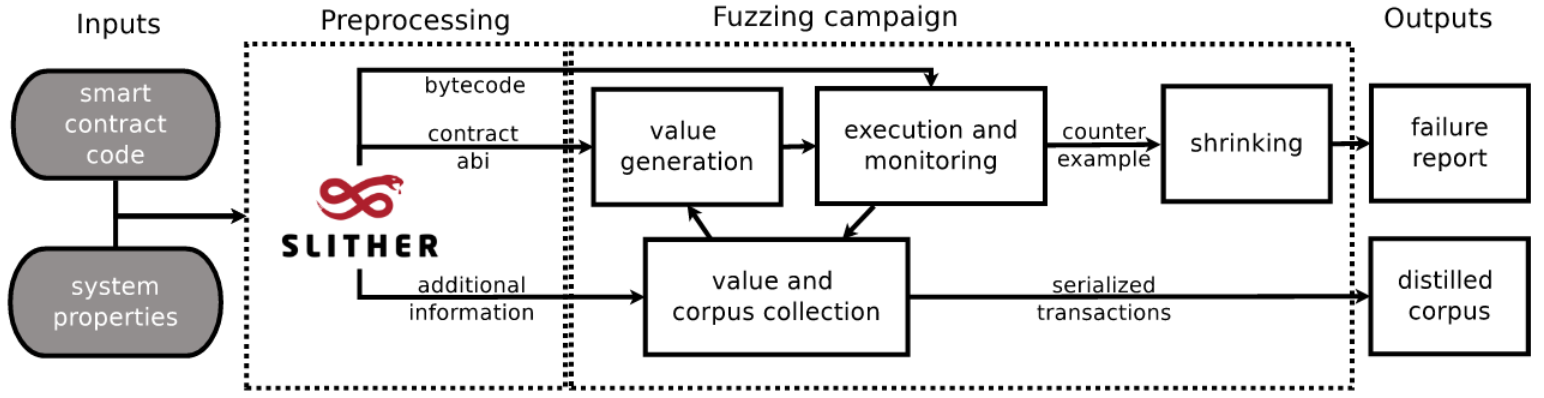
\includegraphics[width=10cm]{logos/echidna.png}
    \caption{Echidna architecture}
    \label{fig:echdina_architecture}
\end{figure}

The code \ref{lst:EchidnaCode} provides an example of invariant in Echdina context. The Solidity contract contains a vulnerability a the backdoor function. The output of the terminal is presented in Listing \ref{lst:EchidnaResult}: the attacker. For breaking the property, can call in order the tunctions airdrops() and backdoor()

\begin{lstlisting} [language=C++, caption={Solidity smart contract implementing a vulnerable Token and an Echidna invariant function.}, label={lst:EchidnaCode}]
contract Token{
    mapping(address => uint) public balances;
    function airdrop() public{
        balances[msg.sender] = 1000;
    }
    function consume() public{
        require(balances[msg.sender]>0);
        balances[msg.sender] -= 1;
    }
    function backdoor() public{
        balances[msg.sender] += 1;
    }
    function echidna_balance_under_1000() public view returns(bool){
        return balances[msg.sender] <= 1000;
    }
}
\end{lstlisting}
\begin{lstlisting} [caption={Tool's result after the execution of the precious code.}, label={lst:EchidnaResult}]
    $ echidna-test testtoken.sol --contract TestToken
    ...
    echidna_balance_under_1000: failed!
    Call sequence, shrinking (1205/5000):
    airdrop()
    backdoor()

    ...
\end{lstlisting}

The tool can be even used to test assertions. 
The aim is equivalent of the invariant testing methodology, 
but in this case properties are expressed using the Solidity annotation of assertion.

\subsection{Solc-Verify}
\label{sec:Specification:Solc-Verify}

\citet{SolcVerify} present solc-verify, a source-level verification tool for
Ethereum smart contracts. It takes smart contracts written
in Solidity and discharges verification conditions using modular program
analysis. It is built on top of the Solidity compiler, so it reasons at the level of the contract source code. 
Becuase of that, Solc-verify is able to reason about high-level contract attributes 
while accurately modeling low-level language semantics.

Solc-verify is implemented as an extension to the Solidity compiler.
It accepts a collection of Solidity contracts, including specification annotations, and uses 
the Boogie verifier and SMT solvers to discharge verification conditions. 

As \citet{SolcVerify_2} explain, Solc-verify translates the annotated contracts to the Boogie Intermediate Verification
Language (IVL). The key idea of the translation is to encode state variables as global heaps
and functions as procedures. Solc-verify relies on the Boogie verifier to perform modular
verification by discharging verification conditions to SMT solvers. The verification conditions
encode the function body while assuming the preconditions, and then check if postconditions
hold. In this process, function calls are replaced by their specification and loops by their
invariants (modularity). Finally, the results are back-annotated to the Solidity source.

\ref{lst:SimpleBank} present an example of annotation, which states that the contract will ensure
that the sum of individual balances is equal to the total balance in the bank.


\begin{lstlisting} [language=C++, caption={An example Solidity smart contract implementing a simple bank with SolcVerify annotations.}, label={lst:SimpleBank}]
pragma solidity >=0.7.0;

/**
 * @notice invariant __verifier_sum_uint(balances) <= address(this).balance
 */
contract SimpleBank {
    mapping(address=>uint) balances;

    function deposit() public payable {
        balances[msg.sender] += msg.value;
    }

    function withdraw(uint256 amount) public {
        require(balances[msg.sender] > amount);
        bool ok;
        (ok, ) = msg.sender.call{value: amount}(""); // Reentrancy attack
        if (!ok) revert();
        balances[msg.sender] -= amount;
    }
}
\end{lstlisting}




\citet{SolcVerify_3} on GitHub repository, present the specification annotations. Those must be included in special documentation comments (/// or /** */) and must start with the special doctag @notice. 
They must be side-effect free Solidity expressions (with some verifier specific extensions) and can refer to variables within the scope of the annotated element. Functions cannot be called in the annotations, except for getters.
The currently available annotations are listed below. 

\begin{itemize}
    \item Function pre/postconditions can be attached to functions. Preconditions are assumed before executing the function and postconditions are checked (asserted) in the end. The expression can refer to variables in the scope of the function. The postcondition can also refer to the return value if it is named.
    \item Contract level invariants can be attached to contracts. They are included as both a pre- and a postcondition for each public function. The expression can refer to state variables in the contract (and its balance).
    \item Loop invariants can be attached to for and while loops. The expression can refer to variables in scope of the loop, including the loop counter.
    \item Modification specifiers can be attached to functions. The target can be a (1) state variable, including index and member accesses or (2) a balance of an address in scope. Note however, that balance changes due to gas cost or miner rewards are currently not modeled.
    \item Event data specification can be attached to events that should be emitted when certain data changes. 
    Events can declare the state variable(s) they track for changes, or in other words, the variables for which the event should be emitted on a change.
\end{itemize}

\section{Tools without specification}
\label{sec:Tools:WithoutSpecification}

\subsection{SmartTest}
\label{sec:WithoutSpecification:SmartTest}

SmartTest is a safety analayzer for Ethereum smart contracts develeoped by \citet{SmartTest}. 
It adopts a symbolic execution technique for effectively detecting vulnerable transaction sequences. 
The main challenge of the project involves the tool to find transaction sequences,
revealing the vulnerabilities of the analysed smart contract. Therefore, bugs are discoved as the cause of the interaction of multiple transactions.
The purpose of SmartTest is to automatically deliver vulnerable transaction sequences, 
which demostrate the weaknesses of the smart contract.
The main idea is to build a statistical model using known vulnerable transaction sequences and use it to direct symbolic execution toward 
more successfully detecting unknown vulnerabilities. 
Symbolic execution is guided by statistical language models, so it can prioritize transacion sequences which are likely to reveal vulenrablities.
This statregy involves firstly to run unguided symbolic
execution on existing vulnerable contracts, then to learn a probablity distribution over vulnerable transaction sequences.

The tool is implemented as an extension of VeriSol, a verifier for Solidity Contracts.
SmartTest is build on top of that, adding its own functionalities:
\begin{itemize}
    \item symbolic execution with a language model.
    \item symbolic executor for transaction sequences.
    \item constraint solving optimization.
\end{itemize}


\subsection{Slither}
\label{sec:WithoutSpecification:Slither}
Slither is described by \citet{Slither} as an open-source static analysis framework.
It uses its own intermediate representation, SlithIR, which was created to simplify static analysis of Solidity code. 
Concolic analysis, taint analysis, and control flow checking are involved for detecting a variety
of security vulnerabilities. It is designed to provide
granular information about smart contract code and the flexibility necessary to support many applications.

It is mainly used for:
\begin{itemize}
    \item Automated vulnerability detection: a large variety of
    smart contract bugs can be detected without user inter-
    vention.
    \item Automated optimization detection: Slither detects code
    optimizations that the compiler misses.
    \item Code understanding: printers summarize and display
    contracts' information to aid in the study of the codebase.
    \item Assisted code review: through its API, a user can interact
    with Slither.
\end{itemize}

Slither implements more than twenty bug detectors, regarding reetrancy, Uninitialized variables,
Shadowing and many other. The tool allows the developers to integrate more detectors, therefore it extends Slither's capabilities
to detect more advanced bugs.

\citet{SlitherGitHub} is written in python 3 and it is published on GitHub.
During the installation, I did not find any particular issues.

\subsection{Mythril}
\label{sec:WithoutSpecification:Mythril}
Mythril is a security analysis tool for Ethereum smart contracts. It was introduced by \citet{Mythril}.

The tool  relies on concolic analysis, taint analysis and control flow checking of the EVM bytecode to
prune the search space and to look for values that allow exploiting
vulnerabilities in the smart contract.
It is targeted at finding common vulnerabilities, 
and is not able to discover issues in the business logic of an application. \citet{SWCRegistry}'s taxonomy of vulnerabilities is used by Mythril for classify them. 
Listig \ref{lst:MythrilOutput} illustrates an example of output of Mythril analysis. 
At the secocond line, there is the reference to the vulnerability classified by SWC Registry with the ID of 110 (Assert Violation).


\begin{lstlisting} [caption={Example of the output of Mythril Analysis.}, label={lst:MythrilOutput}]
==== Exception State ====
SWC ID: 110
Severity: Medium
Contract: Token
Function name: transferArray(address[],uint256[])
PC address: 4385
Estimated Gas Usage: 944 - 6585
An assertion violation was triggered.
It is possible to trigger an assertion violation. Note that Solidity assert() statements should only be used to check invariants. Review the transaction trace generated for this issue and either make sure your program logic is correct, or use require() instead of assert() if your goal is to constrain user inputs or enforce preconditions. Remember to validate inputs from both callers (for instance, via passed arguments) and callees (for instance, via return values).
--------------------
In file: test.sol:309

function transferArray(address[] tos, uint256[] values) public returns (bool) {
        for (uint8 i = 0; i < tos.length; i++) {
            require(transfer(tos[i], values[i]));
        }

        return true;
    }

--------------------

\end{lstlisting}

\subsection{Maian}
\label{sec:WithoutSpecification:Maian}

\subsection{Securify}
\label{sec:WithoutSpecification:Securify}

\subsection{ContractLarva}
\label{sec:WithoutSpecification:ContractLarva}
contractLarva is a runtime verification tool for Solidity contracts. 

\chapter{First Content Chapter}
\label{ch:FirstContent}

%% -------------------
%% | Example content |
%% -------------------
The content chapters of your thesis should of course be renamed. How many
chapters you need to write depends on your thesis and cannot be said in general.

Check out the examples theses in the SDQWiki:

\url{https://sdqweb.ipd.kit.edu/wiki/Hinweise_zu_Abschlussarbeiten#Beispiele_3}

Of course, you can split this .tex file into several files if you prefer. 


\section{First Section}
\label{sec:FirstContent:FirstSection}

\dots

\subsection{A Subsection}
\label{sec:FirstContent:FirstSubSection}

\dots

\subsubsection{A Subsubsection}

\section{Second Section}
\label{sec:FirstContent:SecondSection}

\dots


\chapter{Second Content Chapter}
\label{ch:SecondContent}

\dots

\section{First Section}
\label{sec:SecondContent:FirstSection}

\dots

\section{Second Section}
\label{sec:SecondContent:SecondSection}

\dots

Add additional content chapters if required by adding new .tex files in the
\code{sections/} directory and adding an appropriate 
\code{\textbackslash input} statement in \code{thesis.tex}. 
%% ---------------------
%% | / Example content |
%% ---------------------
